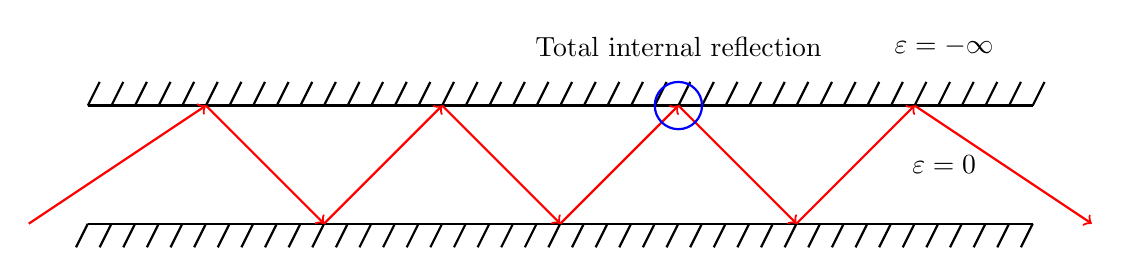
\begin{tikzpicture}[scale=1.5]

% -----------------------------
% Fiber walls (cladding)
% -----------------------------
\draw[thick] (0,0) -- (8,0);   % bottom wall
\draw[thick] (0,1) -- (8,1);   % top wall

% small hatch marks to mimic "/////"
\foreach \x in {0,0.2,...,8} {
    \draw[thick] (\x-0.1,-0.2) -- ++(0.1,0.2);
    \draw[thick] (\x,1) -- ++(0.1, 0.2);
}

% -----------------------------
% Light rays bouncing inside
% -----------------------------
\draw[red, thick, ->] (-0.5,0) -- (1,1);
\draw[red, thick, ->] (1,1) -- (2,0);
\draw[red, thick, ->] (2,0) -- (3,1);
\draw[red, thick, ->] (3,1) -- (4,0);
\draw[red, thick, ->] (4,0) -- (5,1);
\draw[red, thick, ->] (5,1) -- (6,0);
\draw[red, thick, ->] (6,0) -- (7,1);
\draw[red, thick, ->] (7,1) -- (8.5,0);

% note: total internal reflection
  \draw[blue, thick] (5,1) circle (0.2);
  \node at (5,1.5) {Total internal reflection};

\node at (7.25, 1.5) {$\varepsilon=-\infty$};
\node at (7.25, 0.5) {$\varepsilon=0$};

\end{tikzpicture}

